
%(BEGIN_QUESTION)
% Copyright 2006, Tony R. Kuphaldt, released under the Creative Commons Attribution License (v 1.0)
% This means you may do almost anything with this work of mine, so long as you give me proper credit

On processes where the fluid in question is especially dangerous, ``double block-and-bleed'' manifolds are often used to isolate instruments from the process piping.  Consider this example:

$$\includegraphics[width=15.5cm]{i00210x01.eps}$$

Describe the proper procedure for block and bleed valve opening/closing when removing and replacing an instrument connected to a process through such a manifold.

\underbar{file i00210}
%(END_QUESTION)





%(BEGIN_ANSWER)

Removing the gauge from service:

\begin{itemize}
\item{} Close the ``block'' valve closest to the process.
\item{} Open the ``bleed'' valve.  Monitor the instrument's pressure indication, to make sure it is changing to register atmospheric pressure.  This tells you that the ``bleeding'' is successful.
\item{} Close the ``block'' valve closest to the instrument.
\item{} Close the ``bleed'' valve.
\item{} Place lock-out tags on all three valve handles to notify operators and technicians of the instrument's removal and pending return.
\item{} Remove the gauge from the piping or tubing.
\end{itemize}

Assuming the process fluid is especially dangerous, there may be some sort of recommended decontamination process for the instrument prior to you connecting it to calibration equipment in the shop.  As always, be aware of any special safety considerations on any process you are working around.

\vskip 10pt

Placing the gauge back into service:

\begin{itemize}
\item{} Remove the lock-out tags on all valve handles.
\item{} Open the ``bleed'' valve (to relieve any pressure that may have built up between the two closed block valves from a leak in the first block valve).
\item{} Re-attach the gauge to the piping or tubing.
\item{} Open the ``block'' valve closest to the instrument.
\item{} Close the ``bleed'' valve.
\item{} Open the ``block'' valve closest to the process.
\end{itemize}

%(END_ANSWER)





%(BEGIN_NOTES)

Examples of dangerous processes requiring double block/bleed manifolds might include:

\begin{itemize}
\goodbreak
\item{} Highly flammable liquids or gases
\item{} Highly toxic liquid or gases
\item{} High pressure liquids or gases
\item{} Any combination of the above
\end{itemize}

%INDEX% Safety, isolation valves: double block and bleed

%(END_NOTES)


